% Created 2016-08-17 Wed 14:38
\documentclass[tikz]{standalone}

\usepackage[utf8]{inputenc}
\usepackage[T1]{fontenc}

\usepackage{circledsteps}

\RequirePackage{xcolor}

%% HPI color definitions according to the design manual
% These do not exactly match the RGB values used in the Powerpoint slide master due to unknown reasons
\definecolor{hpiyellow}{RGB}{246,168,0}
\definecolor{hpiorange}{RGB}{221,97,8}
\definecolor{hpired}{RGB}{177,6,58}
\definecolor{hpigray}{RGB}{90,96,101}
\definecolor{hpiblue}{RGB}{0,122,158}


\renewcommand{\sfdefault}{neosans}
% Different font weights for neosans
\newcommand{\textl}[1]{{\fontseries{l}\selectfont #1}} % light
\newcommand{\textm}[1]{{\fontseries{m}\selectfont #1}} % medium, same as default weight
\newcommand{\textsb}[1]{{\fontseries{sb}\selectfont #1}} % semibold
\newcommand{\textmb}[1]{{\fontseries{mb}\selectfont #1}} % bold, same as \textbf
\newcommand{\texteb}[1]{{\fontseries{eb}\selectfont #1}} % extra bold
\newcommand{\textub}[1]{{\fontseries{ub}\selectfont #1}} % ultra bold

\tikzset{every picture/.style={/utils/exec={\sffamily}}}
\tikzset{flipflop RSflanke/.style={
  flipflop,
  flipflop def={t1=S, t2=C, c2=1, t3=R, t6=Q, t4={\ctikztextnot{Q}}}
}}


\tikzset{
  mechanicalSwitch/.pic={
    \coordinate (-inUp) at (135:2); 
    \coordinate (-inDown) at (235:2);
    \coordinate (-out) at (2,0);
    \coordinate (-center) at (0,0);
    
    \draw (0,0) circle [radius = 2cm];
    \draw [fill=gray!20] (0,0) circle [radius = 0.2cm];

    \draw (0, 0) -- (2, 0);
    \draw (135:.8) -- (135:2); 
    \draw (225:.8) -- (225:2); 

    \draw [fill=gray!20] (2, 0) circle [radius=0.05cm]; 
    \draw [fill=gray!20] (135:2) circle [radius=0.05cm]; 
    \draw [fill=gray!20] (225:2) circle [radius=0.05cm]; 

    
    \draw [thick] (0,0) -- (175:1.5); 

    \draw [dashed, <->, domain=135:225] plot ({cos(\x)}, {sin(\x)}); 
  },
  mechanicalSwitchClosed/.pic={
    \coordinate (-inUp) at (135:2); 
    \coordinate (-inDown) at (255:2);
    \coordinate (-out) at (2,0);
    \coordinate (-center) at (0,0);
    \draw (0,0) circle [radius = 2cm];
    \draw [fill=gray!20] (0,0) circle [radius = 0.2cm];

    \draw (0, 0) -- (2, 0);
    \draw (135:.8) -- (135:2); 
    \draw (225:.8) -- (225:2); 

    \draw [fill=gray!20] (2, 0) circle [radius=0.05cm]; 
    \draw [fill=gray!20] (135:2) circle [radius=0.05cm]; 
    \draw [fill=gray!20] (225:2) circle [radius=0.05cm]; 

    
    \draw [thick] (0,0) -- (135:2); 

    \draw [dashed, <->, domain=135:225] plot ({cos(\x)}, {sin(\x)}); 
  }
}


\usetikzlibrary{calc}
\usetikzlibrary{positioning}


\usetikzlibrary{ext.positioning-plus,backgrounds,fit,shapes.multipart}


\begin{document}

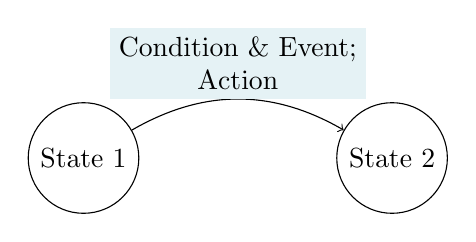
\begin{tikzpicture}
  \node [draw, circle] (s1) {State 1}; 
  \node [draw, circle, right= 2.5cm of s1] (s2) {State 2};

  \draw [->] (s1) to [out=30,in=150] node [above,align=center, fill=hpiblue!10] {Condition \& Event; \\Action} (s2); 
\end{tikzpicture}


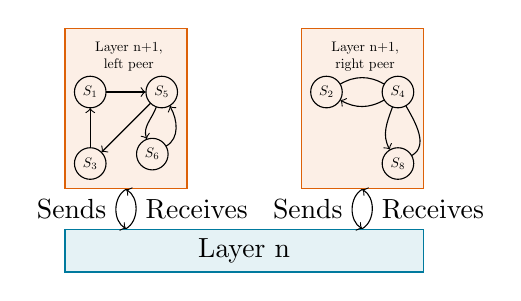
\begin{tikzpicture}
  
  \begin{scope}[scale=0.5, every node/.append style={transform shape}]
    \node [draw, circle] (s1l) {$S_1$}; 
    \node [draw, circle, right=of s1l] (s5l) {$S_5$};
    \node [draw, circle, below=of s1l] (s3l) {$S_3$};
    \node [draw, circle, below right =of s1l] (s6l) {$S_6$};

    \draw [->] (s1l) -- (s5l) edge (s3l) edge [out=250,in=110] (s6l);
    \draw [->] (s6l) to [out=30,in=300] (s5l); 
    \draw [->] (s3l) -- (s1l);
    \node [above=0cm of s1l,anchor=south west,align=center] (fsmllabel) {Layer n+1,\\ left peer};
    
    \begin{scope}[on background layer]
      \node [fit=(s1l)(s5l)(s3l)(s6l)(fsmllabel), draw=hpiorange,fill=hpiorange!10] (fsml) {}; 
    \end{scope}
\end{scope}


  \begin{scope}[scale=0.5, every node/.append style={transform shape},
    xshift=6cm]
    \node [draw, circle] (s2r) {$S_2$}; 
    \node [draw, circle, right=of s2r] (s4r) {$S_4$};
    \node [draw, circle, below=of s4r] (s8r) {$S_8$};

    \draw [->] (s2r) to [out=30,in=150] (s4r) (s4r) to [out=210,in=330] (s2r);
    \draw [->] (s8r) to [out=30,in=300] (s4r) to [out=250,in=120] (s8r);

    \node [above=0cm of s2r,anchor=south west,align=center] (fsmrlabel) {Layer n+1,\\ right peer}; 
    \begin{scope}[on background layer]
      \node [fit=(s2r)(s4r)(s8r)(fsmrlabel), draw=hpiorange,fill=hpiorange!10] (fsmr) {}; 
    \end{scope}
\end{scope}

  
  \node [fill=hpiblue!10,draw=hpiblue, below=0.5cm of -(fsml)(fsmr)] (ln) {Layer n}; 
  \draw [->] (fsml.south) to [out=210,in=150] node [left] {Sends} (fsml |- ln.north);
  \draw [->] (fsml.south |- ln.north) to [out=30,in=330]  node [right] {Receives} (fsml.south) ;
  \draw [->] (fsmr.south) to [out=210,in=150] node [left] {Sends} (fsmr |- ln.north);
  \draw [->] (fsmr.south |- ln.north) to [out=30,in=330]  node [right] {Receives} (fsmr.south) ;

  
\end{tikzpicture}

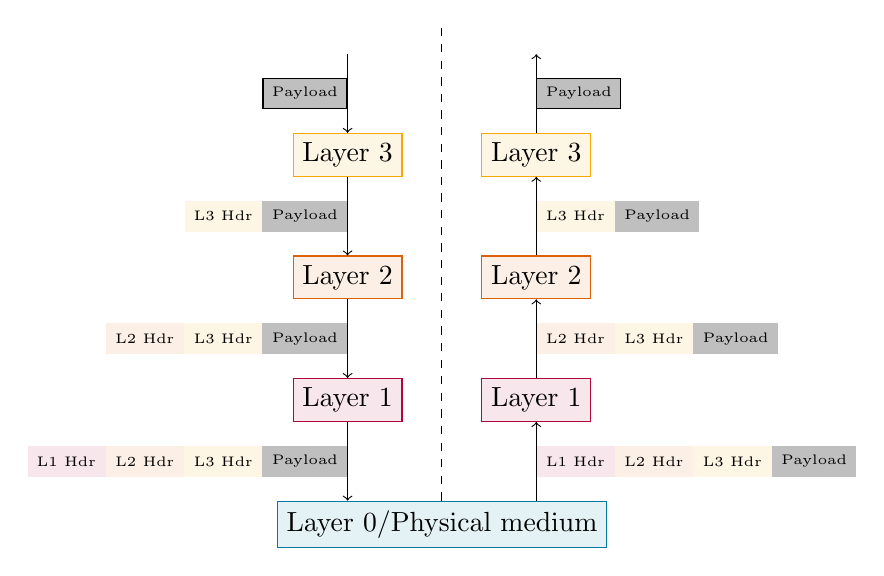
\begin{tikzpicture}
  \label{page:basics:headers}
  \node [fill=hpiyellow!10,draw=hpiyellow] (l3l) {Layer 3};
  \node [fill=hpiyellow!10,draw=hpiyellow, right=of l3l] (l3r) {Layer 3};
  
  \node [fill=hpiorange!10,draw=hpiorange, below=of l3l] (l2l) {Layer 2};
  \node [fill=hpiorange!10,draw=hpiorange, right=of l2l] (l2r) {Layer 2};

  \node [fill=hpired!10,draw=hpired, below=of l2l] (l1l) {Layer 1};
  \node [fill=hpired!10,draw=hpired, right=of l1l] (l1r) {Layer 1};

  \node [fill=hpiblue!10, draw=hpiblue, below=of -(l1l)(l1r)] (l0) {Layer 0/Physical medium};

  \draw [->] ([yshift=1cm]l3l.north) to
  node [left,fill=gray!50, draw, minimum width=0.5] {\tiny Payload}
  (l3l);
  \draw [->] (l3l) to
  node [left, anchor=east, 
  rectangle split, rectangle split horizontal, rectangle split parts=2,
  rectangle split part fill={hpiyellow!10,gray!50},
  ] {\tiny L3 Hdr \nodepart{two} \tiny Payload }
  (l2l);
  \draw [->] (l2l) to
  node [left, anchor=east, 
  rectangle split, rectangle split horizontal, rectangle split parts=3,
  rectangle split part fill={hpiorange!10,hpiyellow!10,gray!50},
  ] {\tiny L2 Hdr \nodepart{two} \tiny L3 Hdr \nodepart{three} \tiny Payload }
  (l1l);
  \draw [->] (l1l)  to
  node [left, anchor=east, 
  rectangle split, rectangle split horizontal, rectangle split parts=4,
  rectangle split part fill={hpired!10,hpiorange!10,hpiyellow!10,gray!50},
  ] {\tiny L1 Hdr \nodepart{two} \tiny L2 Hdr \nodepart{three} \tiny L3 Hdr \nodepart{four} \tiny Payload }
  (l0.north -| l1l); 
  
  \draw [<-] ([yshift=1cm]l3r.north)  to
  node [right,fill=gray!50, draw, minimum width=0.5] {\tiny Payload} (l3r); 
  \draw [<-] (l3r)  to
  node [right, anchor=west, 
  rectangle split, rectangle split horizontal, rectangle split parts=2,
  rectangle split part fill={hpiyellow!10,gray!50},
  ] {\tiny L3 Hdr \nodepart{two} \tiny Payload }
  (l2r);
  \draw [<-] (l2r)  to
  node [right, anchor=west, 
  rectangle split, rectangle split horizontal, rectangle split parts=3,
  rectangle split part fill={hpiorange!10,hpiyellow!10,gray!50},
  ] {\tiny L2 Hdr \nodepart{two} \tiny L3 Hdr \nodepart{three} \tiny Payload } (l1r);
  \draw [<-] (l1r)  to
  node [right, anchor=west, 
  rectangle split, rectangle split horizontal, rectangle split parts=4,
  rectangle split part fill={hpired!10,hpiorange!10,hpiyellow!10,gray!50},
  ] {\tiny L1 Hdr \nodepart{two} \tiny L2 Hdr \nodepart{three} \tiny L3 Hdr \nodepart{four} \tiny Payload } (l0.north -| l1r); 

  \draw [dashed] (l0.north) -- ++ (0,6); 
  
\end{tikzpicture}


\end{document} 